\documentclass[preprint, 10pt]{aastex}
\usepackage{newtxtext, newtxmath}

\usepackage{graphicx}
\graphicspath{
  {../},
}

\newcommand\oiii{[\ion{O}{3}]}
\newcommand\nii{[\ion{N}{2}]}
\newcommand\sii{[\ion{S}{2}]}
\newcommand\elec{\ensuremath{_{\mathrm{e}}}}
\newcommand\Te{\ensuremath{T\elec}}
\newcommand\Ne{\ensuremath{n\elec}}

\usepackage{geometry}
\geometry{margin=1in}
\setkeys{Gin}{width=0.6\linewidth, keepaspectratio}  

\usepackage{natbib}
\usepackage{microtype}
\bibliographystyle{apj}


\newcommand\Pixel{\ensuremath{\Omega_{\mathrm{pix}}}}
\newcommand\Area{\ensuremath{A_{\mathrm{HST}}}}
\newcommand\T[2]{\ensuremath{T_{#1}^{#2}}}
\newcommand\Tlam[1]{\T{\lambda}{#1}}
\newcommand\Tmax[1]{\T{\mathrm{m}}{#1}}
\newcommand\Mean[1]{\ensuremath{\bigl\langle \lambda I_\lambda \bigr\rangle_{#1}}}
\newcommand\MeanC[1]{\ensuremath{\bigl\langle \lambda
    I_\lambda^{\mathrm{cont}} \bigr\rangle_{#1}}}
\newcommand\Color[2]{\ensuremath{k_{#1, #2}}}
\newcommand\COLOR[2]{\ensuremath{\widetilde{k}_{#1, #2}}}
\newcommand\Weff[2]{\ensuremath{\widetilde{W}_{#1, #2}}}
\newcommand\U[1]{\ensuremath{\mathrm{#1}}}
\newcommand\E[1]{\ensuremath{\times 10^{#1}}}
\newcommand\Elam{\ensuremath{\varepsilon_\lambda}}
\newcommand\Constant{\ensuremath{C_{\mathrm{WFC3}}}}


% \newcommand\Narrow{\mathrm{L}}
% \newcommand\Wide{\mathrm{C}}
% \newcommand\Narrow{\mathrm{a}}
% \newcommand\Wide{\mathrm{b}}
\newcommand\Narrow{\mathrm{N}}
\newcommand\Wide{\mathrm{W}}
\newcommand\Contam{\ensuremath{{i'}}} %extra braces are on purpose

\begin{document}

\section{Temperature and density fluctuations in the inner Orion Nebula}
\label{sec:fluct}



\subsection{Deriving diagnostic line ratios from WFC3 filter images}
\label{sec:filters}
\begin{figure}
  \centering
  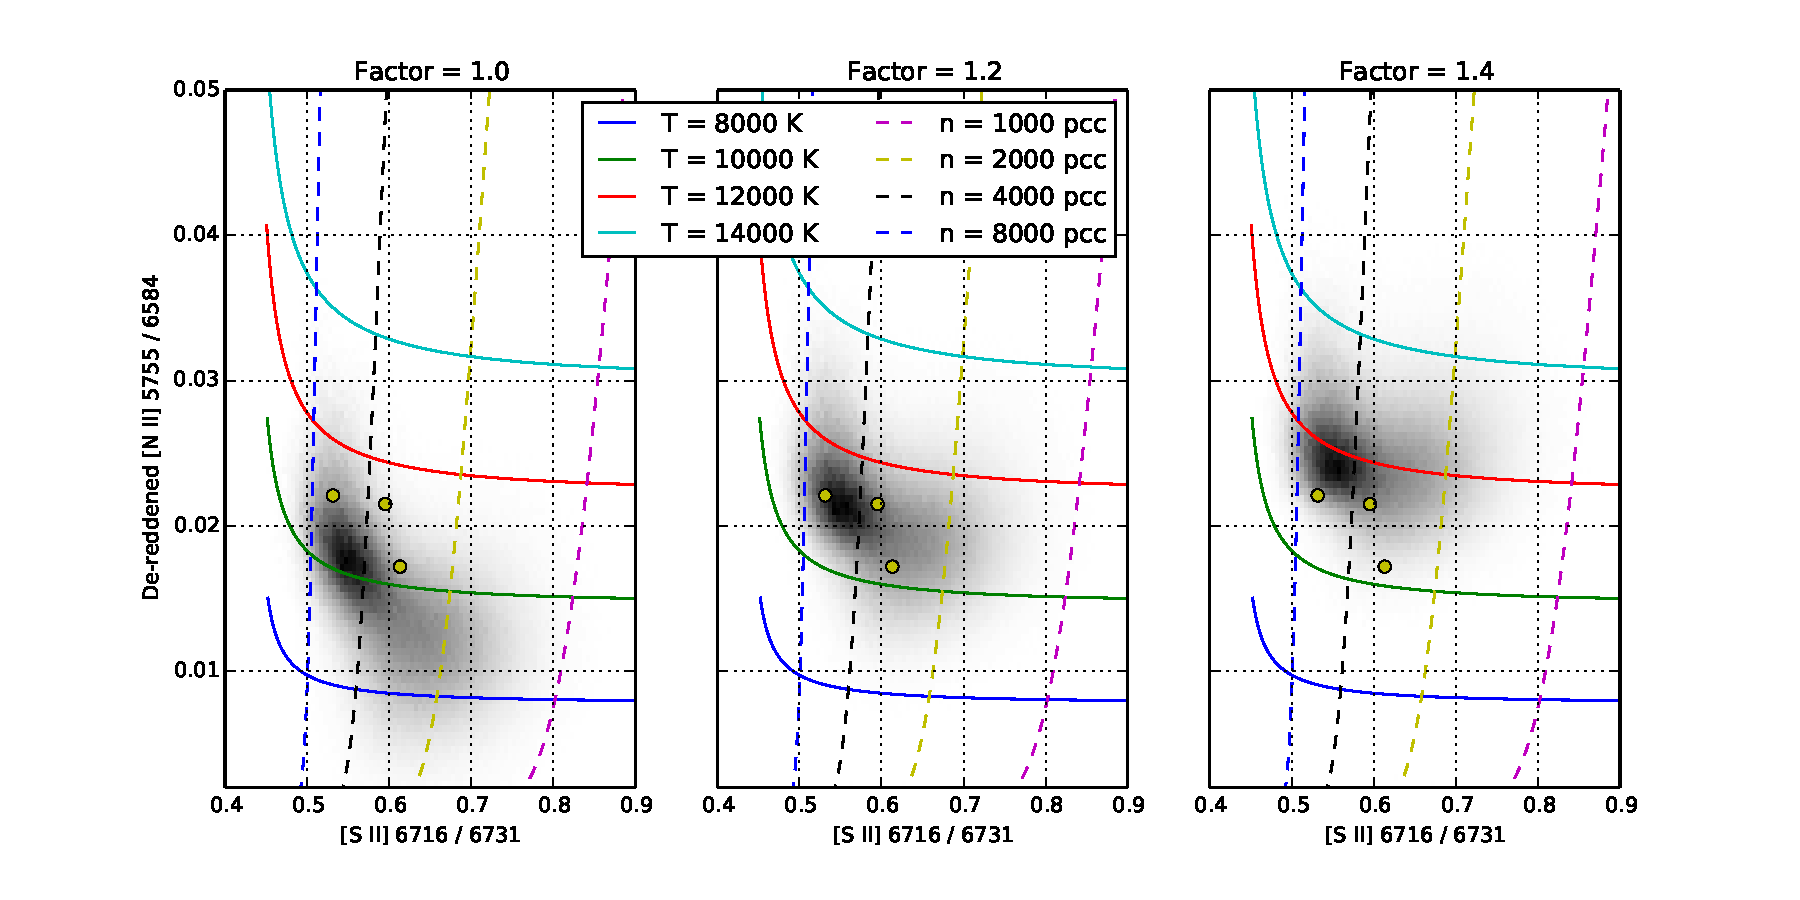
\includegraphics[width=\linewidth]{bivar_rsii_rnii_multifactor}
  \caption{Distribution of line ratios}
  \label{fig:line-ratios}
\end{figure}

\textit{Note: this is similar to what I wrote in the the calibration
  draft, but specifically tailored to line ratios rather than
  equivalent widths.}

The WFC3 camera is equipped with filters that effectively target
important nebular diagnostic lines.  Each filter, with label \(j\), is
characterized by an effective transmission profile, or throughput,
\Tlam{j}, which gives the wavelength-dependent conversion factor
between the number of photons arriving at the \textit{HST} entrance
aperture (nominal radius: \(120\ \U{cm}\)) and the number of electrons
registered by the CCD, accounting for occultation by the secondary
mirror, all other optical and quantum efficiencies, and the amplifier
gain.  The peak value of the filter transmission profile is denoted
\Tmax{j}, with typical values of 0.2--0.3, and the ``rectangular
width'' of the profile is defined as
\begin{equation}
  \label{eq:width}
  W_j = (\Tmax{j})^{-1} \int_0^\infty \!\!\Tlam{j}\, d\lambda 
  \quad\quad [W_j] = \U{\AA}.
\end{equation}


Extensive and continuing on-orbit calibration of the filters has been
carried out (\textit{citation of relevant ISRs}) using white dwarf
standard stars.  However, since these are flat featureless continuum
sources, the calibration is only sensitive to the product \(W_j
\Tmax{j}\).  Emission lines from photoionized regions are
intrinsically much narrower than even the narrowest WFC3 filters, so
the transmission of such a line, with label \(i\), is independent of
\Tlam{j} and depends instead on the throughput at the line wavelength:
\(\T{i}{j} \equiv \Tlam{j}(\lambda\!=\!\lambda_i)\), which has only
been measured pre-launch.   


The calibration of these filters
is discussed in detail in a companion paper \citep{Henney:Calib},
where it is 

For the strongest lines, such as
\nii{6583} 
In order to accurately calculate emission line ratios from WFC3
images, it is important to properly account for the contamination 


\subsection{\boldmath Deriving \(\Te, \Ne\) from line ratios}
\label{sec:derive}

\begin{figure}
  \centering
  \begin{tabular}{ll}
    (\textit{a}) & (\textit{b}) \\
    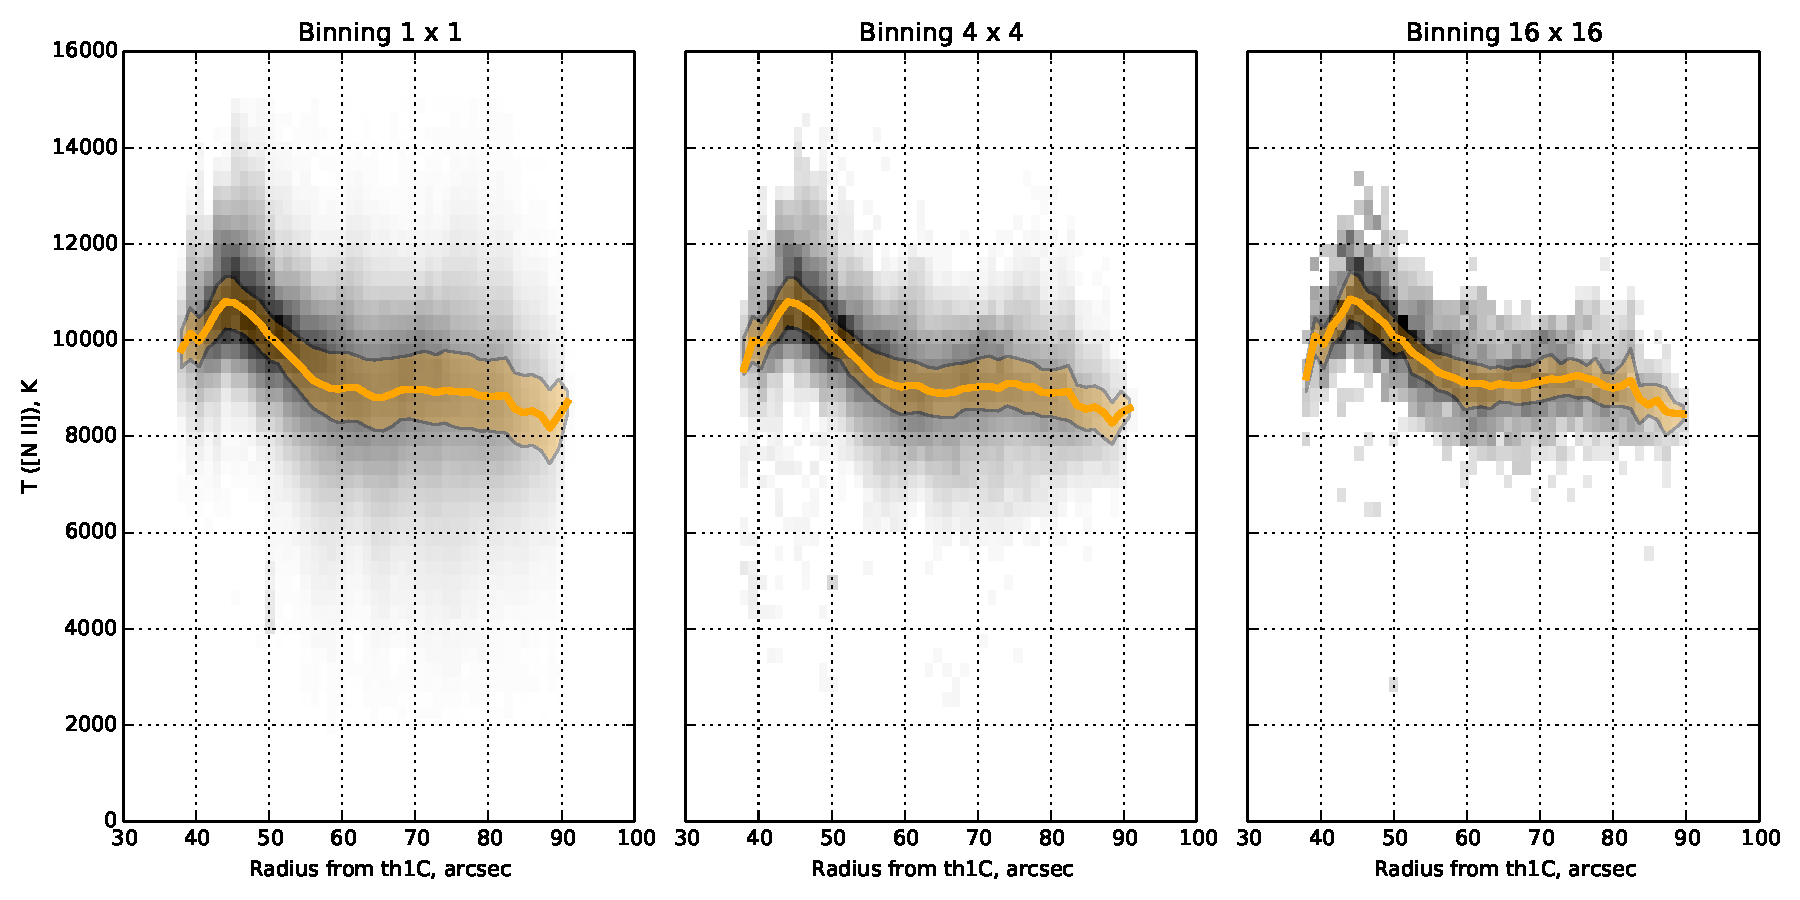
\includegraphics[height=0.35\textheight]{Tnii-vs-radius-binning} &
    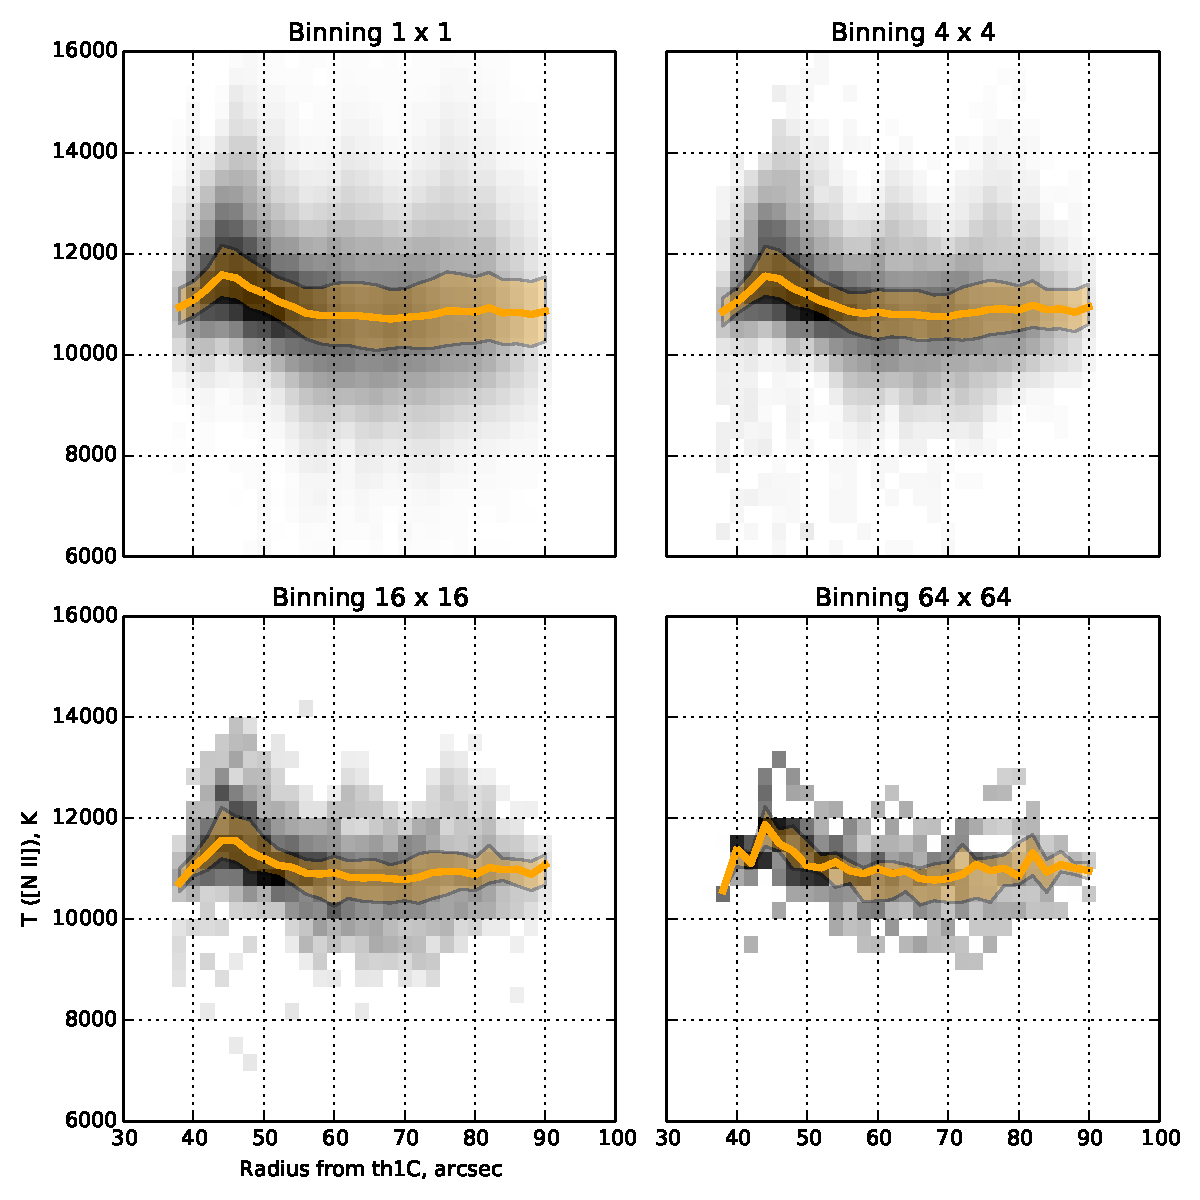
\includegraphics[height=0.25\textheight]{sigma-Tnii-vs-radius-binning}
  \end{tabular}
  \caption{(\textit{a})~Temperature distribution as a function of
    radius for different binnings.  (\textit{b})~Standard deviation of
    temperatures as a function of radius for different binnings. 
  }
  \label{fig:tnii-vs-rad}
\end{figure}


\subsection{\boldmath Analysis of fluctuations in \(\Te, \Ne\)}
\label{sec:fluct}


\begin{figure}
  \centering

  \begin{tabular}{ll}
    (\textit{a}) & (\textit{b}) \\
    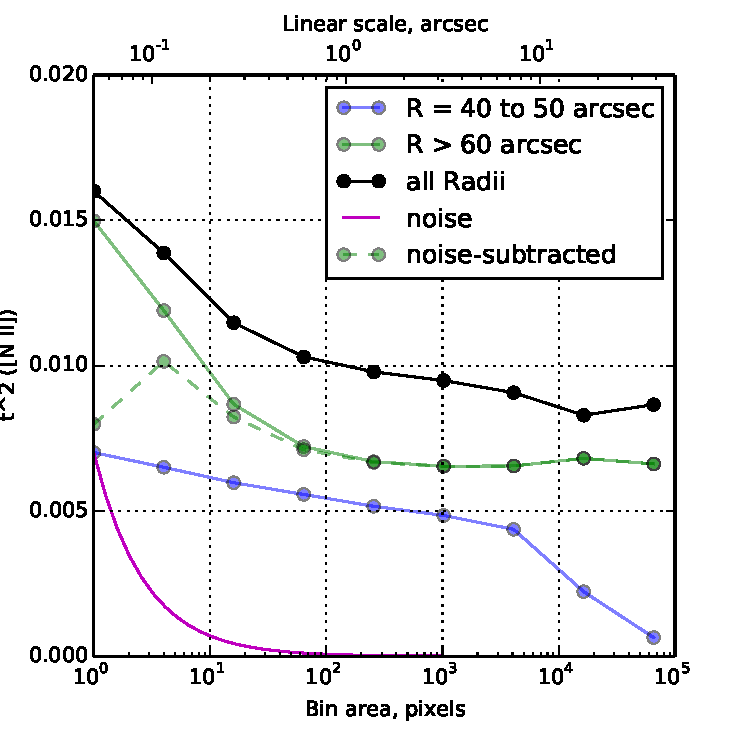
\includegraphics[width=0.45\linewidth]{Tsq-nii-vs-binning-normal} &
    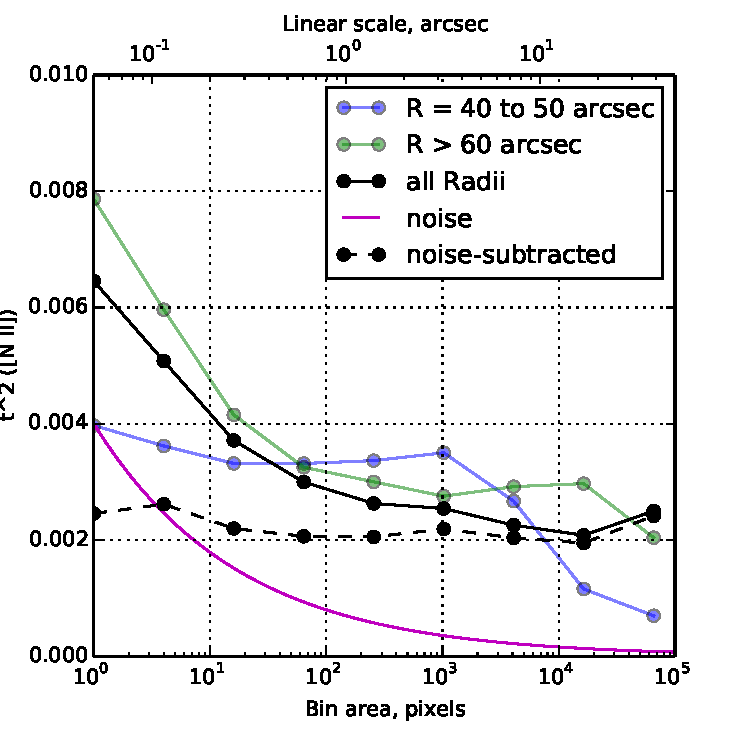
\includegraphics[width=0.45\linewidth]{Tsq-nii-vs-binning-robust}
  \end{tabular}
  \caption{Scale-dependence of temperature fluctuations: \(t^2\) as a
    function of binning. (\textit{a})~Variance of \(\Te/\bar{\Te}\)
    for the entire image (black line) and two subsamples: an annulus
    centered on the high-temperature region (blue line) and the more
    distant, fainter regions (green line).  The magenta line is an
    estimate of the noise contribution to the full sample, and the
    dashed black line is the result of subtracting the noise from the
    observed values.  (\textit{b})~Same as \textit{a} but using a
    ``robust'' estimator of the variance, based on the interquartile range.}
  \label{fig:tsq-nii-vs-binning}
\end{figure}


\begin{figure}
  \centering
  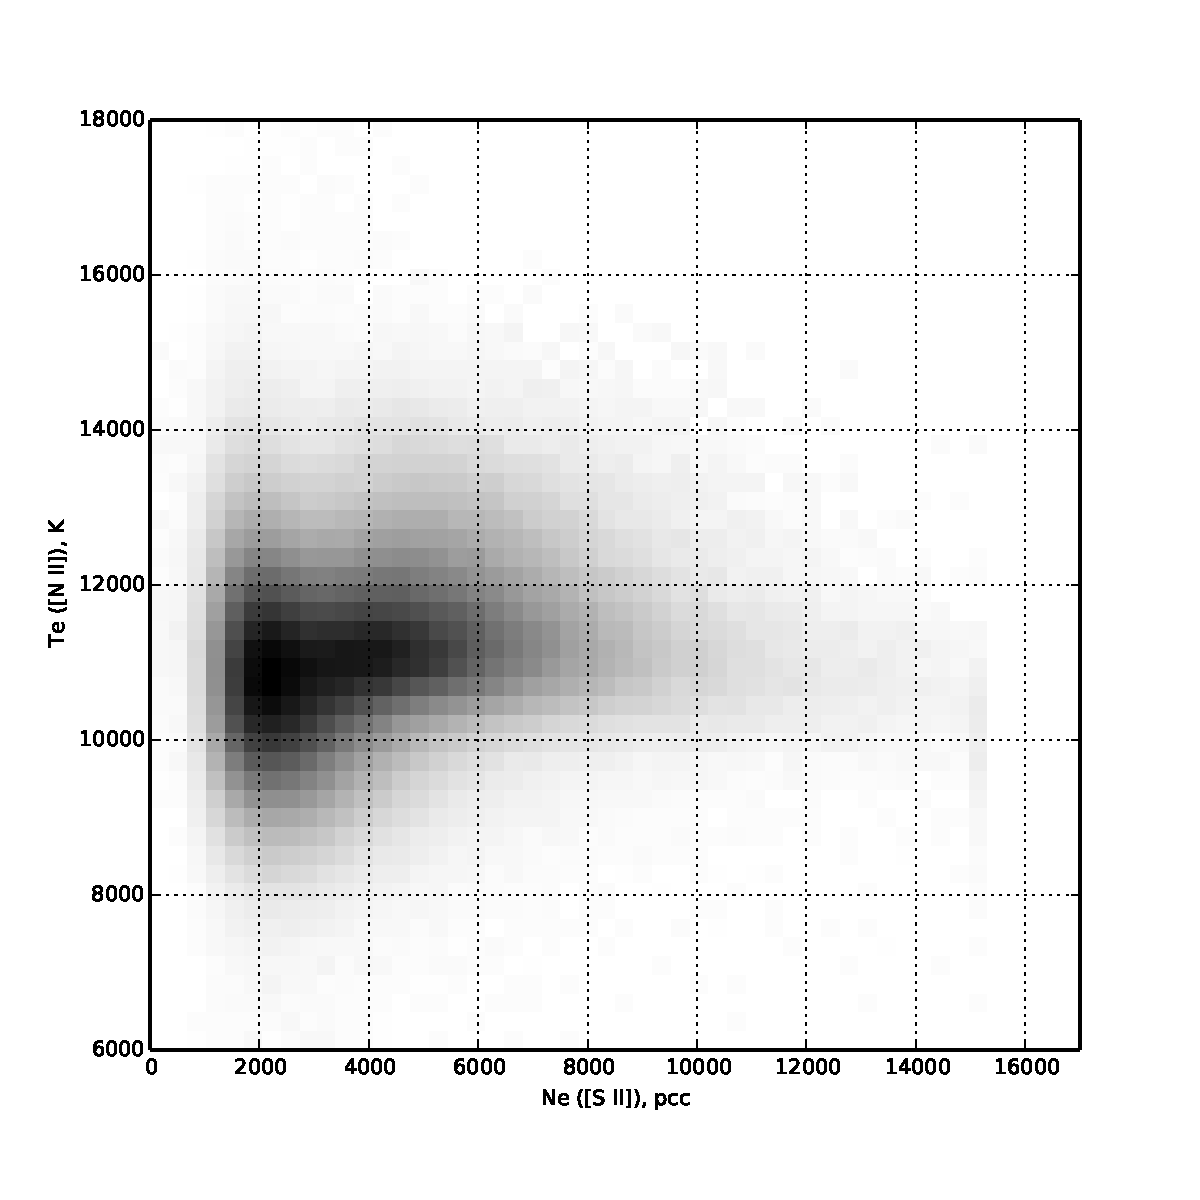
\includegraphics[width=0.8\linewidth]{Te-versus-Ne}
  \caption{Joint distribution of temperature and electron density for
    low ionization regions.}
  \label{fig:Te-Ne}
\end{figure}

\begin{figure}
  \centering
  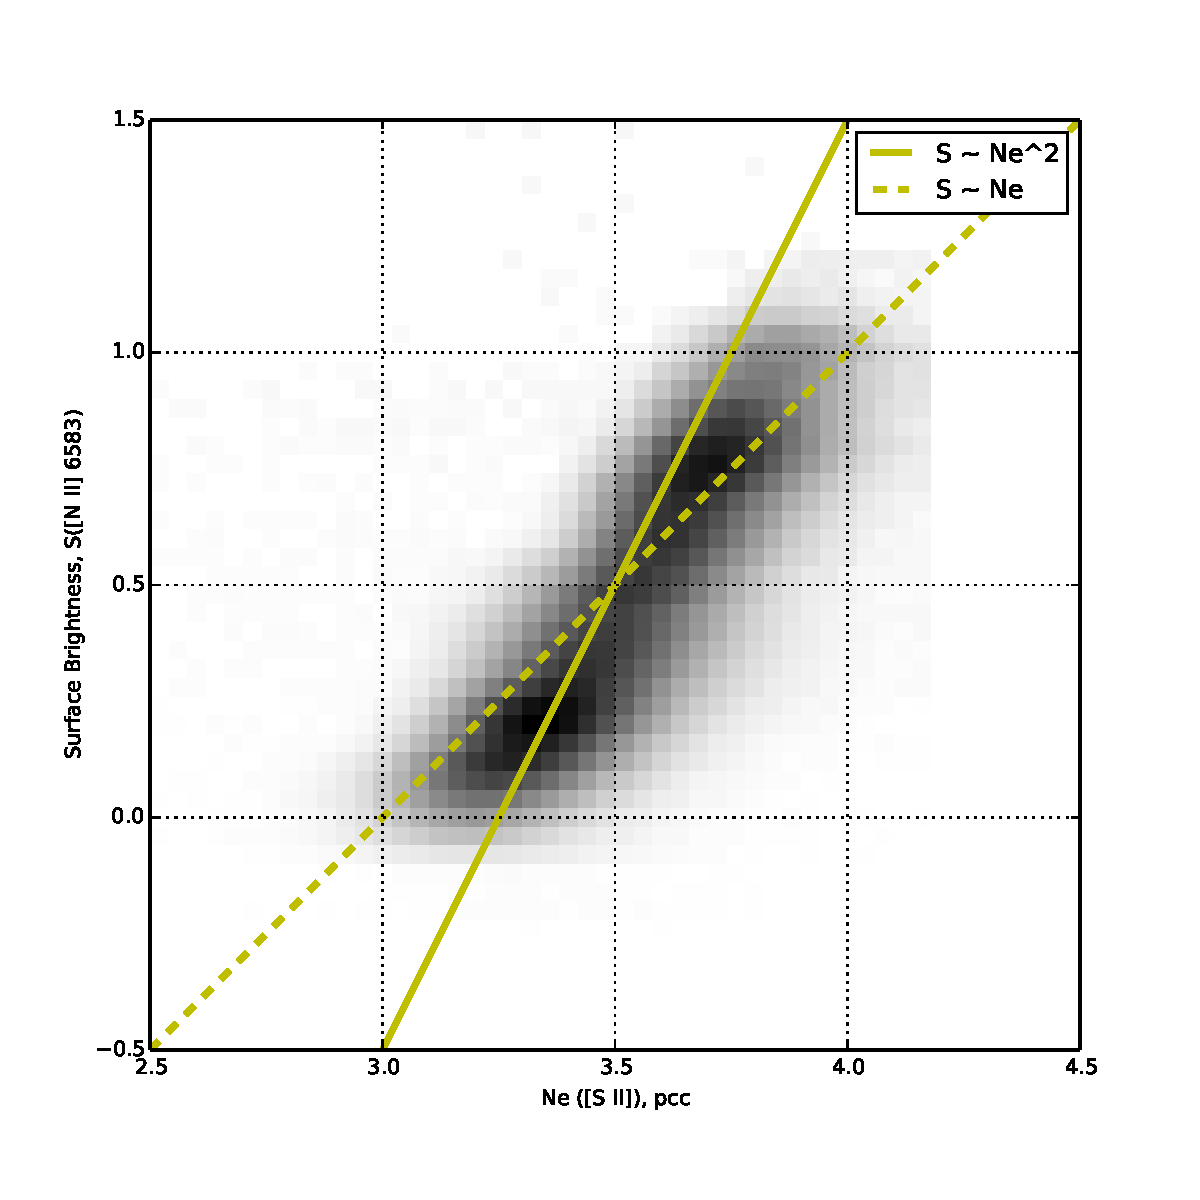
\includegraphics[width=0.8\linewidth]{snii-versus-ne}
  \caption{Correlation between \sii{} density and \nii{} surface brightness.}
  \label{fig:Snii-ne}
\end{figure}


\bibliography{BibdeskLibrary-slavoj}


\end{document}
